% SOURCE: ../../edit-harness/results/frame_a/cells/cell_*_real_MIX_A_*.json
% !TEX encoding = UTF-8 Unicode
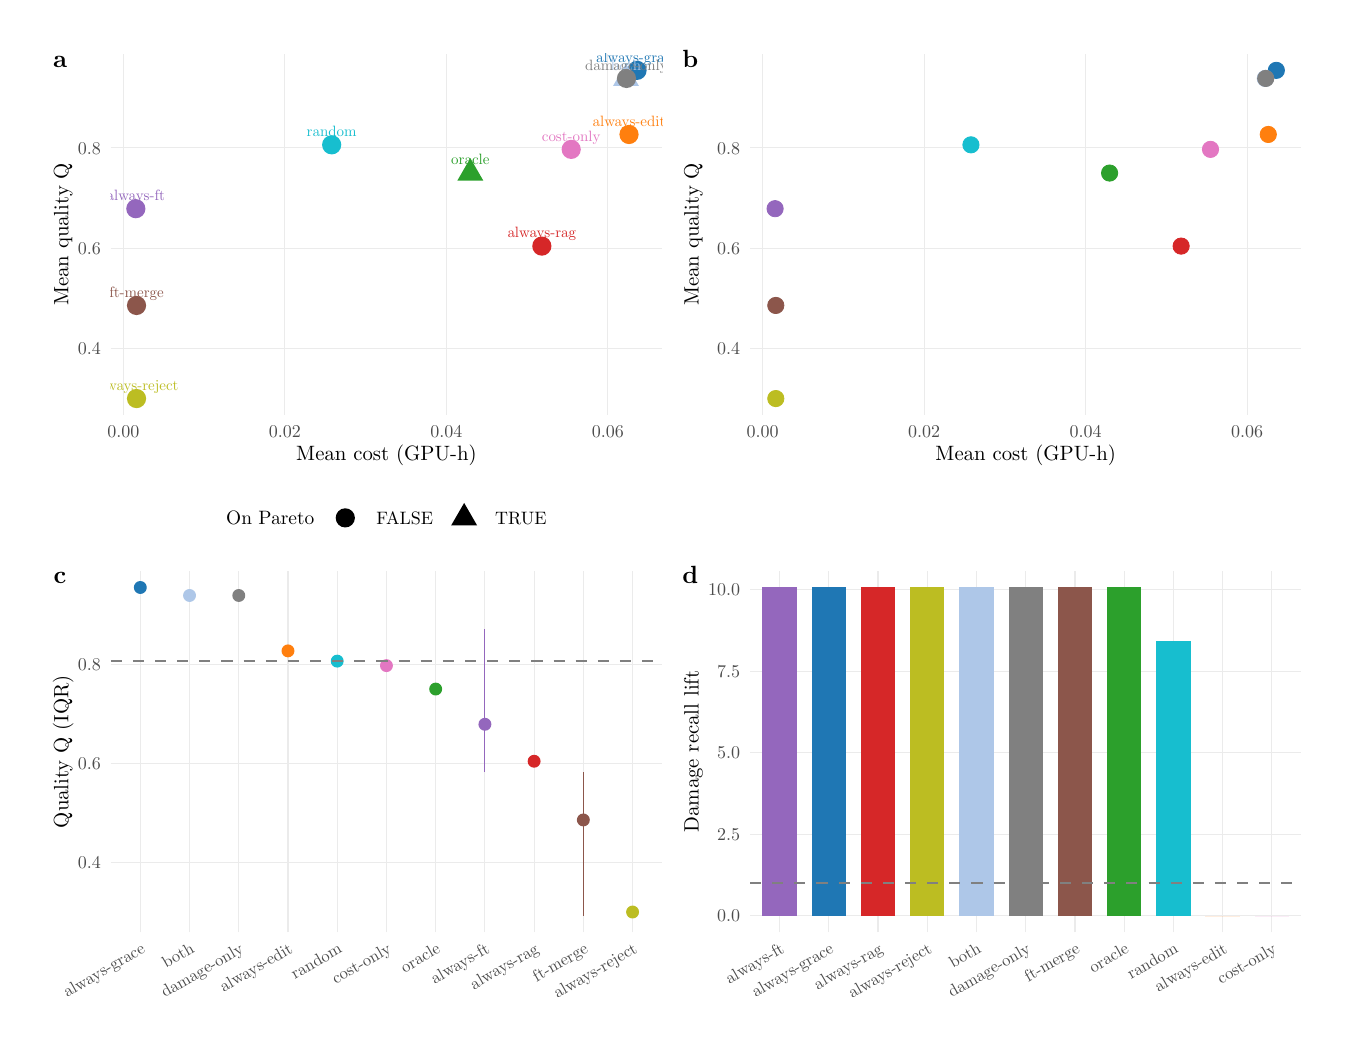
\begin{tikzpicture}[x=1pt,y=1pt]
\definecolor{fillColor}{RGB}{255,255,255}
\path[use as bounding box,fill=fillColor,fill opacity=0.00] (0,0) rectangle (469.75,361.35);
\begin{scope}
\path[clip] (  0.00,  0.00) rectangle (469.75,361.35);
\definecolor{drawColor}{RGB}{255,255,255}
\definecolor{fillColor}{RGB}{255,255,255}

\path[draw=drawColor,line width= 0.6pt,line join=round,line cap=round,fill=fillColor] (  0.00,  0.00) rectangle (469.76,361.35);
\end{scope}
\begin{scope}
\path[clip] (  5.50,168.99) rectangle (233.25,355.85);
\definecolor{fillColor}{RGB}{255,255,255}

\path[fill=fillColor] (  5.50,168.99) rectangle (233.25,355.85);
\end{scope}
\begin{scope}
\path[clip] (233.25,168.99) rectangle (464.25,355.85);
\definecolor{fillColor}{RGB}{255,255,255}

\path[fill=fillColor] (233.25,168.99) rectangle (464.25,355.85);
\end{scope}
\begin{scope}
\path[clip] (  5.50,  5.50) rectangle (233.25,168.99);
\definecolor{fillColor}{RGB}{255,255,255}

\path[fill=fillColor] (  5.50,  5.50) rectangle (233.25,168.99);
\end{scope}
\begin{scope}
\path[clip] (233.25,  5.50) rectangle (464.25,168.99);
\definecolor{fillColor}{RGB}{255,255,255}

\path[fill=fillColor] (233.25,  5.50) rectangle (464.25,168.99);
\end{scope}
\begin{scope}
\path[clip] ( 30.03,221.41) rectangle (229.25,351.85);
\definecolor{drawColor}{gray}{0.92}

\path[draw=drawColor,line width= 0.4pt,line join=round] ( 30.03,245.46) --
	(229.25,245.46);

\path[draw=drawColor,line width= 0.4pt,line join=round] ( 30.03,281.70) --
	(229.25,281.70);

\path[draw=drawColor,line width= 0.4pt,line join=round] ( 30.03,317.94) --
	(229.25,317.94);

\path[draw=drawColor,line width= 0.4pt,line join=round] ( 34.54,221.41) --
	( 34.54,351.85);

\path[draw=drawColor,line width= 0.4pt,line join=round] ( 92.91,221.41) --
	( 92.91,351.85);

\path[draw=drawColor,line width= 0.4pt,line join=round] (151.28,221.41) --
	(151.28,351.85);

\path[draw=drawColor,line width= 0.4pt,line join=round] (209.65,221.41) --
	(209.65,351.85);
\definecolor{fillColor}{RGB}{255,127,14}

\path[fill=fillColor] (217.29,322.76) circle (  3.47);
\definecolor{fillColor}{RGB}{148,103,189}

\path[fill=fillColor] ( 39.08,295.94) circle (  3.47);
\definecolor{fillColor}{RGB}{31,119,180}

\path[fill=fillColor] (220.20,345.92) circle (  3.47);
\definecolor{fillColor}{RGB}{214,39,40}

\path[fill=fillColor] (185.79,282.42) circle (  3.47);
\definecolor{fillColor}{RGB}{188,189,34}

\path[fill=fillColor] ( 39.33,227.33) circle (  3.47);
\definecolor{fillColor}{RGB}{174,199,232}

\path[fill=fillColor] (216.20,348.40) --
	(220.87,340.30) --
	(211.52,340.30) --
	cycle;
\definecolor{fillColor}{RGB}{227,119,194}

\path[fill=fillColor] (196.40,317.37) circle (  3.47);
\definecolor{fillColor}{gray}{0.50}

\path[fill=fillColor] (216.37,343.00) circle (  3.47);
\definecolor{fillColor}{RGB}{140,86,75}

\path[fill=fillColor] ( 39.33,260.97) circle (  3.47);
\definecolor{fillColor}{RGB}{44,160,44}

\path[fill=fillColor] (159.95,314.21) --
	(164.62,306.11) --
	(155.27,306.11) --
	cycle;
\definecolor{fillColor}{RGB}{23,190,207}

\path[fill=fillColor] (109.85,319.01) circle (  3.47);
\definecolor{drawColor}{RGB}{255,127,14}

\node[text=drawColor,anchor=base,inner sep=0pt, outer sep=0pt, scale=  0.54] at (217.29,325.74) {always-edit};
\definecolor{drawColor}{RGB}{148,103,189}

\node[text=drawColor,anchor=base,inner sep=0pt, outer sep=0pt, scale=  0.54] at ( 39.08,298.92) {always-ft};
\definecolor{drawColor}{RGB}{31,119,180}

\node[text=drawColor,anchor=base,inner sep=0pt, outer sep=0pt, scale=  0.54] at (220.20,348.90) {always-grace};
\definecolor{drawColor}{RGB}{214,39,40}

\node[text=drawColor,anchor=base,inner sep=0pt, outer sep=0pt, scale=  0.54] at (185.79,285.40) {always-rag};
\definecolor{drawColor}{RGB}{188,189,34}

\node[text=drawColor,anchor=base,inner sep=0pt, outer sep=0pt, scale=  0.54] at ( 39.33,230.31) {always-reject};
\definecolor{drawColor}{RGB}{174,199,232}

\node[text=drawColor,anchor=base,inner sep=0pt, outer sep=0pt, scale=  0.54] at (216.20,345.98) {both};
\definecolor{drawColor}{RGB}{227,119,194}

\node[text=drawColor,anchor=base,inner sep=0pt, outer sep=0pt, scale=  0.54] at (196.40,320.35) {cost-only};
\definecolor{drawColor}{gray}{0.50}

\node[text=drawColor,anchor=base,inner sep=0pt, outer sep=0pt, scale=  0.54] at (216.37,345.98) {damage-only};
\definecolor{drawColor}{RGB}{140,86,75}

\node[text=drawColor,anchor=base,inner sep=0pt, outer sep=0pt, scale=  0.54] at ( 39.33,263.95) {ft-merge};
\definecolor{drawColor}{RGB}{44,160,44}

\node[text=drawColor,anchor=base,inner sep=0pt, outer sep=0pt, scale=  0.54] at (159.95,311.79) {oracle};
\definecolor{drawColor}{RGB}{23,190,207}

\node[text=drawColor,anchor=base,inner sep=0pt, outer sep=0pt, scale=  0.54] at (109.85,321.99) {random};
\end{scope}
\begin{scope}
\path[clip] (  0.00,  0.00) rectangle (469.75,361.35);
\definecolor{drawColor}{gray}{0.30}

\node[text=drawColor,anchor=base east,inner sep=0pt, outer sep=0pt, scale=  0.65] at ( 26.43,243.22) {0.4};

\node[text=drawColor,anchor=base east,inner sep=0pt, outer sep=0pt, scale=  0.65] at ( 26.43,279.46) {0.6};

\node[text=drawColor,anchor=base east,inner sep=0pt, outer sep=0pt, scale=  0.65] at ( 26.43,315.70) {0.8};
\end{scope}
\begin{scope}
\path[clip] (  0.00,  0.00) rectangle (469.75,361.35);
\definecolor{drawColor}{gray}{0.30}

\node[text=drawColor,anchor=base,inner sep=0pt, outer sep=0pt, scale=  0.65] at ( 34.54,213.33) {0.00};

\node[text=drawColor,anchor=base,inner sep=0pt, outer sep=0pt, scale=  0.65] at ( 92.91,213.33) {0.02};

\node[text=drawColor,anchor=base,inner sep=0pt, outer sep=0pt, scale=  0.65] at (151.28,213.33) {0.04};

\node[text=drawColor,anchor=base,inner sep=0pt, outer sep=0pt, scale=  0.65] at (209.65,213.33) {0.06};
\end{scope}
\begin{scope}
\path[clip] (  0.00,  0.00) rectangle (469.75,361.35);
\definecolor{drawColor}{RGB}{0,0,0}

\node[text=drawColor,anchor=base,inner sep=0pt, outer sep=0pt, scale=  0.75] at (129.64,204.90) {Mean cost (GPU-h)};
\end{scope}
\begin{scope}
\path[clip] (  0.00,  0.00) rectangle (469.75,361.35);
\definecolor{drawColor}{RGB}{0,0,0}

\node[text=drawColor,rotate= 90.00,anchor=base,inner sep=0pt, outer sep=0pt, scale=  0.75] at ( 14.67,286.63) {Mean quality Q};
\end{scope}
\begin{scope}
\path[clip] (  0.00,  0.00) rectangle (469.75,361.35);
\definecolor{drawColor}{RGB}{0,0,0}

\node[text=drawColor,anchor=base west,inner sep=0pt, outer sep=0pt, scale=  0.70] at ( 71.74,181.80) {On Pareto};
\end{scope}
\begin{scope}
\path[clip] (  0.00,  0.00) rectangle (469.75,361.35);
\definecolor{fillColor}{RGB}{0,0,0}

\path[fill=fillColor] (114.77,184.21) circle (  3.47);
\end{scope}
\begin{scope}
\path[clip] (  0.00,  0.00) rectangle (469.75,361.35);
\definecolor{fillColor}{RGB}{0,0,0}

\path[fill=fillColor] (157.72,189.61) --
	(162.39,181.52) --
	(153.04,181.52) --
	cycle;
\end{scope}
\begin{scope}
\path[clip] (  0.00,  0.00) rectangle (469.75,361.35);
\definecolor{drawColor}{RGB}{0,0,0}

\node[text=drawColor,anchor=base west,inner sep=0pt, outer sep=0pt, scale=  0.65] at (126.00,181.98) {FALSE};
\end{scope}
\begin{scope}
\path[clip] (  0.00,  0.00) rectangle (469.75,361.35);
\definecolor{drawColor}{RGB}{0,0,0}

\node[text=drawColor,anchor=base west,inner sep=0pt, outer sep=0pt, scale=  0.65] at (168.94,181.98) {TRUE};
\end{scope}
\begin{scope}
\path[clip] (  0.00,  0.00) rectangle (469.75,361.35);
\definecolor{drawColor}{RGB}{0,0,0}

\node[text=drawColor,anchor=base,inner sep=0pt, outer sep=0pt, scale=  0.90] at ( 11.70,346.96) {\bfseries a};
\end{scope}
\begin{scope}
\path[clip] (261.03,221.41) rectangle (460.25,351.85);
\definecolor{drawColor}{gray}{0.92}

\path[draw=drawColor,line width= 0.4pt,line join=round] (261.03,245.46) --
	(460.25,245.46);

\path[draw=drawColor,line width= 0.4pt,line join=round] (261.03,281.70) --
	(460.25,281.70);

\path[draw=drawColor,line width= 0.4pt,line join=round] (261.03,317.94) --
	(460.25,317.94);

\path[draw=drawColor,line width= 0.4pt,line join=round] (265.54,221.41) --
	(265.54,351.85);

\path[draw=drawColor,line width= 0.4pt,line join=round] (323.91,221.41) --
	(323.91,351.85);

\path[draw=drawColor,line width= 0.4pt,line join=round] (382.28,221.41) --
	(382.28,351.85);

\path[draw=drawColor,line width= 0.4pt,line join=round] (440.65,221.41) --
	(440.65,351.85);
\definecolor{drawColor}{RGB}{255,127,14}
\definecolor{fillColor}{RGB}{255,127,14}

\path[draw=drawColor,line width= 0.3pt,line join=round,line cap=round,fill=fillColor] (448.29,322.76) circle (  2.94);
\definecolor{drawColor}{RGB}{148,103,189}
\definecolor{fillColor}{RGB}{148,103,189}

\path[draw=drawColor,line width= 0.3pt,line join=round,line cap=round,fill=fillColor] (270.08,295.94) circle (  2.94);
\definecolor{drawColor}{RGB}{31,119,180}
\definecolor{fillColor}{RGB}{31,119,180}

\path[draw=drawColor,line width= 0.3pt,line join=round,line cap=round,fill=fillColor] (451.20,345.92) circle (  2.94);
\definecolor{drawColor}{RGB}{214,39,40}
\definecolor{fillColor}{RGB}{214,39,40}

\path[draw=drawColor,line width= 0.3pt,line join=round,line cap=round,fill=fillColor] (416.80,282.42) circle (  2.94);
\definecolor{drawColor}{RGB}{188,189,34}
\definecolor{fillColor}{RGB}{188,189,34}

\path[draw=drawColor,line width= 0.3pt,line join=round,line cap=round,fill=fillColor] (270.33,227.33) circle (  2.94);
\definecolor{drawColor}{RGB}{174,199,232}
\definecolor{fillColor}{RGB}{174,199,232}

\path[draw=drawColor,line width= 0.3pt,line join=round,line cap=round,fill=fillColor] (447.20,343.00) circle (  2.94);
\definecolor{drawColor}{RGB}{227,119,194}
\definecolor{fillColor}{RGB}{227,119,194}

\path[draw=drawColor,line width= 0.3pt,line join=round,line cap=round,fill=fillColor] (427.41,317.37) circle (  2.94);
\definecolor{drawColor}{gray}{0.50}
\definecolor{fillColor}{gray}{0.50}

\path[draw=drawColor,line width= 0.3pt,line join=round,line cap=round,fill=fillColor] (447.37,343.00) circle (  2.94);
\definecolor{drawColor}{RGB}{140,86,75}
\definecolor{fillColor}{RGB}{140,86,75}

\path[draw=drawColor,line width= 0.3pt,line join=round,line cap=round,fill=fillColor] (270.33,260.97) circle (  2.94);
\definecolor{drawColor}{RGB}{44,160,44}
\definecolor{fillColor}{RGB}{44,160,44}

\path[draw=drawColor,line width= 0.3pt,line join=round,line cap=round,fill=fillColor] (390.95,308.81) circle (  2.94);
\definecolor{drawColor}{RGB}{23,190,207}
\definecolor{fillColor}{RGB}{23,190,207}

\path[draw=drawColor,line width= 0.3pt,line join=round,line cap=round,fill=fillColor] (340.85,319.01) circle (  2.94);
\end{scope}
\begin{scope}
\path[clip] (  0.00,  0.00) rectangle (469.75,361.35);
\definecolor{drawColor}{gray}{0.30}

\node[text=drawColor,anchor=base east,inner sep=0pt, outer sep=0pt, scale=  0.65] at (257.43,243.22) {0.4};

\node[text=drawColor,anchor=base east,inner sep=0pt, outer sep=0pt, scale=  0.65] at (257.43,279.46) {0.6};

\node[text=drawColor,anchor=base east,inner sep=0pt, outer sep=0pt, scale=  0.65] at (257.43,315.70) {0.8};
\end{scope}
\begin{scope}
\path[clip] (  0.00,  0.00) rectangle (469.75,361.35);
\definecolor{drawColor}{gray}{0.30}

\node[text=drawColor,anchor=base,inner sep=0pt, outer sep=0pt, scale=  0.65] at (265.54,213.33) {0.00};

\node[text=drawColor,anchor=base,inner sep=0pt, outer sep=0pt, scale=  0.65] at (323.91,213.33) {0.02};

\node[text=drawColor,anchor=base,inner sep=0pt, outer sep=0pt, scale=  0.65] at (382.28,213.33) {0.04};

\node[text=drawColor,anchor=base,inner sep=0pt, outer sep=0pt, scale=  0.65] at (440.65,213.33) {0.06};
\end{scope}
\begin{scope}
\path[clip] (  0.00,  0.00) rectangle (469.75,361.35);
\definecolor{drawColor}{RGB}{0,0,0}

\node[text=drawColor,anchor=base,inner sep=0pt, outer sep=0pt, scale=  0.75] at (360.64,204.90) {Mean cost (GPU-h)};
\end{scope}
\begin{scope}
\path[clip] (  0.00,  0.00) rectangle (469.75,361.35);
\definecolor{drawColor}{RGB}{0,0,0}

\node[text=drawColor,rotate= 90.00,anchor=base,inner sep=0pt, outer sep=0pt, scale=  0.75] at (242.42,286.63) {Mean quality Q};
\end{scope}
\begin{scope}
\path[clip] (  0.00,  0.00) rectangle (469.75,361.35);
\definecolor{drawColor}{RGB}{0,0,0}

\node[text=drawColor,anchor=base,inner sep=0pt, outer sep=0pt, scale=  0.90] at (239.48,346.96) {\bfseries b};
\end{scope}
\begin{scope}
\path[clip] ( 30.03, 34.54) rectangle (229.25,164.99);
\definecolor{drawColor}{gray}{0.92}

\path[draw=drawColor,line width= 0.4pt,line join=round] ( 30.03, 59.71) --
	(229.25, 59.71);

\path[draw=drawColor,line width= 0.4pt,line join=round] ( 30.03, 95.55) --
	(229.25, 95.55);

\path[draw=drawColor,line width= 0.4pt,line join=round] ( 30.03,131.39) --
	(229.25,131.39);

\path[draw=drawColor,line width= 0.4pt,line join=round] ( 40.70, 34.54) --
	( 40.70,164.99);

\path[draw=drawColor,line width= 0.4pt,line join=round] ( 58.49, 34.54) --
	( 58.49,164.99);

\path[draw=drawColor,line width= 0.4pt,line join=round] ( 76.28, 34.54) --
	( 76.28,164.99);

\path[draw=drawColor,line width= 0.4pt,line join=round] ( 94.06, 34.54) --
	( 94.06,164.99);

\path[draw=drawColor,line width= 0.4pt,line join=round] (111.85, 34.54) --
	(111.85,164.99);

\path[draw=drawColor,line width= 0.4pt,line join=round] (129.64, 34.54) --
	(129.64,164.99);

\path[draw=drawColor,line width= 0.4pt,line join=round] (147.43, 34.54) --
	(147.43,164.99);

\path[draw=drawColor,line width= 0.4pt,line join=round] (165.22, 34.54) --
	(165.22,164.99);

\path[draw=drawColor,line width= 0.4pt,line join=round] (183.00, 34.54) --
	(183.00,164.99);

\path[draw=drawColor,line width= 0.4pt,line join=round] (200.79, 34.54) --
	(200.79,164.99);

\path[draw=drawColor,line width= 0.4pt,line join=round] (218.58, 34.54) --
	(218.58,164.99);
\definecolor{drawColor}{RGB}{255,127,14}

\path[draw=drawColor,line width= 0.4pt,line join=round] ( 94.06,135.00) -- ( 94.06,137.88);
\definecolor{drawColor}{RGB}{148,103,189}

\path[draw=drawColor,line width= 0.4pt,line join=round] (165.22, 92.34) -- (165.22,144.22);
\definecolor{drawColor}{RGB}{31,119,180}

\path[draw=drawColor,line width= 0.4pt,line join=round] ( 40.70,159.06) -- ( 40.70,159.06);
\definecolor{drawColor}{RGB}{214,39,40}

\path[draw=drawColor,line width= 0.4pt,line join=round] (183.00, 96.27) -- (183.00, 96.27);
\definecolor{drawColor}{RGB}{188,189,34}

\path[draw=drawColor,line width= 0.4pt,line join=round] (218.58, 41.79) -- (218.58, 41.79);
\definecolor{drawColor}{RGB}{174,199,232}

\path[draw=drawColor,line width= 0.4pt,line join=round] ( 58.49,155.00) -- ( 58.49,158.40);
\definecolor{drawColor}{RGB}{227,119,194}

\path[draw=drawColor,line width= 0.4pt,line join=round] (129.64,129.24) -- (129.64,132.62);
\definecolor{drawColor}{gray}{0.50}

\path[draw=drawColor,line width= 0.4pt,line join=round] ( 76.28,155.00) -- ( 76.28,158.40);
\definecolor{drawColor}{RGB}{140,86,75}

\path[draw=drawColor,line width= 0.4pt,line join=round] (200.79, 40.47) -- (200.79, 92.36);
\definecolor{drawColor}{RGB}{44,160,44}

\path[draw=drawColor,line width= 0.4pt,line join=round] (147.43,122.14) -- (147.43,122.57);
\definecolor{drawColor}{RGB}{23,190,207}

\path[draw=drawColor,line width= 0.4pt,line join=round] (111.85,132.12) -- (111.85,133.00);
\definecolor{drawColor}{RGB}{255,127,14}
\definecolor{fillColor}{RGB}{255,127,14}

\path[draw=drawColor,line width= 0.5pt,line join=round,line cap=round,fill=fillColor] ( 94.06,136.15) circle (  2.08);
\definecolor{drawColor}{RGB}{148,103,189}
\definecolor{fillColor}{RGB}{148,103,189}

\path[draw=drawColor,line width= 0.5pt,line join=round,line cap=round,fill=fillColor] (165.22,109.63) circle (  2.08);
\definecolor{drawColor}{RGB}{31,119,180}
\definecolor{fillColor}{RGB}{31,119,180}

\path[draw=drawColor,line width= 0.5pt,line join=round,line cap=round,fill=fillColor] ( 40.70,159.06) circle (  2.08);
\definecolor{drawColor}{RGB}{214,39,40}
\definecolor{fillColor}{RGB}{214,39,40}

\path[draw=drawColor,line width= 0.5pt,line join=round,line cap=round,fill=fillColor] (183.00, 96.27) circle (  2.08);
\definecolor{drawColor}{RGB}{188,189,34}
\definecolor{fillColor}{RGB}{188,189,34}

\path[draw=drawColor,line width= 0.5pt,line join=round,line cap=round,fill=fillColor] (218.58, 41.79) circle (  2.08);
\definecolor{drawColor}{RGB}{174,199,232}
\definecolor{fillColor}{RGB}{174,199,232}

\path[draw=drawColor,line width= 0.5pt,line join=round,line cap=round,fill=fillColor] ( 58.49,156.17) circle (  2.08);
\definecolor{drawColor}{RGB}{227,119,194}
\definecolor{fillColor}{RGB}{227,119,194}

\path[draw=drawColor,line width= 0.5pt,line join=round,line cap=round,fill=fillColor] (129.64,130.83) circle (  2.08);
\definecolor{drawColor}{gray}{0.50}
\definecolor{fillColor}{gray}{0.50}

\path[draw=drawColor,line width= 0.5pt,line join=round,line cap=round,fill=fillColor] ( 76.28,156.17) circle (  2.08);
\definecolor{drawColor}{RGB}{140,86,75}
\definecolor{fillColor}{RGB}{140,86,75}

\path[draw=drawColor,line width= 0.5pt,line join=round,line cap=round,fill=fillColor] (200.79, 75.06) circle (  2.08);
\definecolor{drawColor}{RGB}{44,160,44}
\definecolor{fillColor}{RGB}{44,160,44}

\path[draw=drawColor,line width= 0.5pt,line join=round,line cap=round,fill=fillColor] (147.43,122.36) circle (  2.08);
\definecolor{drawColor}{RGB}{23,190,207}
\definecolor{fillColor}{RGB}{23,190,207}

\path[draw=drawColor,line width= 0.5pt,line join=round,line cap=round,fill=fillColor] (111.85,132.45) circle (  2.08);
\definecolor{drawColor}{gray}{0.50}

\path[draw=drawColor,line width= 0.5pt,dash pattern=on 4pt off 4pt ,line join=round] ( 30.03,132.45) -- (229.25,132.45);
\end{scope}
\begin{scope}
\path[clip] (  0.00,  0.00) rectangle (469.75,361.35);
\definecolor{drawColor}{gray}{0.30}

\node[text=drawColor,anchor=base east,inner sep=0pt, outer sep=0pt, scale=  0.65] at ( 26.43, 57.47) {0.4};

\node[text=drawColor,anchor=base east,inner sep=0pt, outer sep=0pt, scale=  0.65] at ( 26.43, 93.31) {0.6};

\node[text=drawColor,anchor=base east,inner sep=0pt, outer sep=0pt, scale=  0.65] at ( 26.43,129.15) {0.8};
\end{scope}
\begin{scope}
\path[clip] (  0.00,  0.00) rectangle (469.75,361.35);
\definecolor{drawColor}{gray}{0.30}

\node[text=drawColor,rotate= 30.00,anchor=base east,inner sep=0pt, outer sep=0pt, scale=  0.60] at ( 42.77, 27.36) {always-grace};

\node[text=drawColor,rotate= 30.00,anchor=base east,inner sep=0pt, outer sep=0pt, scale=  0.60] at ( 60.55, 27.36) {both};

\node[text=drawColor,rotate= 30.00,anchor=base east,inner sep=0pt, outer sep=0pt, scale=  0.60] at ( 78.34, 27.36) {damage-only};

\node[text=drawColor,rotate= 30.00,anchor=base east,inner sep=0pt, outer sep=0pt, scale=  0.60] at ( 96.13, 27.36) {always-edit};

\node[text=drawColor,rotate= 30.00,anchor=base east,inner sep=0pt, outer sep=0pt, scale=  0.60] at (113.92, 27.36) {random};

\node[text=drawColor,rotate= 30.00,anchor=base east,inner sep=0pt, outer sep=0pt, scale=  0.60] at (131.71, 27.36) {cost-only};

\node[text=drawColor,rotate= 30.00,anchor=base east,inner sep=0pt, outer sep=0pt, scale=  0.60] at (149.49, 27.36) {oracle};

\node[text=drawColor,rotate= 30.00,anchor=base east,inner sep=0pt, outer sep=0pt, scale=  0.60] at (167.28, 27.36) {always-ft};

\node[text=drawColor,rotate= 30.00,anchor=base east,inner sep=0pt, outer sep=0pt, scale=  0.60] at (185.07, 27.36) {always-rag};

\node[text=drawColor,rotate= 30.00,anchor=base east,inner sep=0pt, outer sep=0pt, scale=  0.60] at (202.86, 27.36) {ft-merge};

\node[text=drawColor,rotate= 30.00,anchor=base east,inner sep=0pt, outer sep=0pt, scale=  0.60] at (220.65, 27.36) {always-reject};
\end{scope}
\begin{scope}
\path[clip] (  0.00,  0.00) rectangle (469.75,361.35);
\definecolor{drawColor}{RGB}{0,0,0}

\node[text=drawColor,rotate= 90.00,anchor=base,inner sep=0pt, outer sep=0pt, scale=  0.75] at ( 14.67, 99.77) {Quality Q (IQR)};
\end{scope}
\begin{scope}
\path[clip] (  0.00,  0.00) rectangle (469.75,361.35);
\definecolor{drawColor}{RGB}{0,0,0}

\node[text=drawColor,anchor=base,inner sep=0pt, outer sep=0pt, scale=  0.90] at ( 11.70,160.33) {\bfseries c};
\end{scope}
\begin{scope}
\path[clip] (261.03, 34.54) rectangle (460.25,164.99);
\definecolor{drawColor}{gray}{0.92}

\path[draw=drawColor,line width= 0.4pt,line join=round] (261.03, 40.47) --
	(460.25, 40.47);

\path[draw=drawColor,line width= 0.4pt,line join=round] (261.03, 69.91) --
	(460.25, 69.91);

\path[draw=drawColor,line width= 0.4pt,line join=round] (261.03, 99.35) --
	(460.25, 99.35);

\path[draw=drawColor,line width= 0.4pt,line join=round] (261.03,128.79) --
	(460.25,128.79);

\path[draw=drawColor,line width= 0.4pt,line join=round] (261.03,158.23) --
	(460.25,158.23);

\path[draw=drawColor,line width= 0.4pt,line join=round] (271.70, 34.54) --
	(271.70,164.99);

\path[draw=drawColor,line width= 0.4pt,line join=round] (289.49, 34.54) --
	(289.49,164.99);

\path[draw=drawColor,line width= 0.4pt,line join=round] (307.28, 34.54) --
	(307.28,164.99);

\path[draw=drawColor,line width= 0.4pt,line join=round] (325.07, 34.54) --
	(325.07,164.99);

\path[draw=drawColor,line width= 0.4pt,line join=round] (342.85, 34.54) --
	(342.85,164.99);

\path[draw=drawColor,line width= 0.4pt,line join=round] (360.64, 34.54) --
	(360.64,164.99);

\path[draw=drawColor,line width= 0.4pt,line join=round] (378.43, 34.54) --
	(378.43,164.99);

\path[draw=drawColor,line width= 0.4pt,line join=round] (396.22, 34.54) --
	(396.22,164.99);

\path[draw=drawColor,line width= 0.4pt,line join=round] (414.01, 34.54) --
	(414.01,164.99);

\path[draw=drawColor,line width= 0.4pt,line join=round] (431.79, 34.54) --
	(431.79,164.99);

\path[draw=drawColor,line width= 0.4pt,line join=round] (449.58, 34.54) --
	(449.58,164.99);
\definecolor{fillColor}{RGB}{255,127,14}

\path[fill=fillColor] (425.57, 40.47) rectangle (438.02, 40.47);
\definecolor{fillColor}{RGB}{148,103,189}

\path[fill=fillColor] (265.48, 40.47) rectangle (277.93,159.06);
\definecolor{fillColor}{RGB}{31,119,180}

\path[fill=fillColor] (283.26, 40.47) rectangle (295.72,159.06);
\definecolor{fillColor}{RGB}{214,39,40}

\path[fill=fillColor] (301.05, 40.47) rectangle (313.50,159.06);
\definecolor{fillColor}{RGB}{188,189,34}

\path[fill=fillColor] (318.84, 40.47) rectangle (331.29,159.06);
\definecolor{fillColor}{RGB}{174,199,232}

\path[fill=fillColor] (336.63, 40.47) rectangle (349.08,159.06);
\definecolor{fillColor}{RGB}{227,119,194}

\path[fill=fillColor] (443.36, 40.47) rectangle (455.81, 40.47);
\definecolor{fillColor}{gray}{0.50}

\path[fill=fillColor] (354.42, 40.47) rectangle (366.87,159.06);
\definecolor{fillColor}{RGB}{140,86,75}

\path[fill=fillColor] (372.20, 40.47) rectangle (384.66,159.06);
\definecolor{fillColor}{RGB}{44,160,44}

\path[fill=fillColor] (389.99, 40.47) rectangle (402.44,159.06);
\definecolor{fillColor}{RGB}{23,190,207}

\path[fill=fillColor] (407.78, 40.47) rectangle (420.23,139.86);
\definecolor{drawColor}{gray}{0.50}

\path[draw=drawColor,line width= 0.5pt,dash pattern=on 4pt off 4pt ,line join=round] (261.03, 52.25) -- (460.25, 52.25);
\end{scope}
\begin{scope}
\path[clip] (  0.00,  0.00) rectangle (469.75,361.35);
\definecolor{drawColor}{gray}{0.30}

\node[text=drawColor,anchor=base east,inner sep=0pt, outer sep=0pt, scale=  0.65] at (257.43, 38.23) {0.0};

\node[text=drawColor,anchor=base east,inner sep=0pt, outer sep=0pt, scale=  0.65] at (257.43, 67.67) {2.5};

\node[text=drawColor,anchor=base east,inner sep=0pt, outer sep=0pt, scale=  0.65] at (257.43, 97.11) {5.0};

\node[text=drawColor,anchor=base east,inner sep=0pt, outer sep=0pt, scale=  0.65] at (257.43,126.55) {7.5};

\node[text=drawColor,anchor=base east,inner sep=0pt, outer sep=0pt, scale=  0.65] at (257.43,155.99) {10.0};
\end{scope}
\begin{scope}
\path[clip] (  0.00,  0.00) rectangle (469.75,361.35);
\definecolor{drawColor}{gray}{0.30}

\node[text=drawColor,rotate= 30.00,anchor=base east,inner sep=0pt, outer sep=0pt, scale=  0.60] at (273.77, 27.36) {always-ft};

\node[text=drawColor,rotate= 30.00,anchor=base east,inner sep=0pt, outer sep=0pt, scale=  0.60] at (291.56, 27.36) {always-grace};

\node[text=drawColor,rotate= 30.00,anchor=base east,inner sep=0pt, outer sep=0pt, scale=  0.60] at (309.34, 27.36) {always-rag};

\node[text=drawColor,rotate= 30.00,anchor=base east,inner sep=0pt, outer sep=0pt, scale=  0.60] at (327.13, 27.36) {always-reject};

\node[text=drawColor,rotate= 30.00,anchor=base east,inner sep=0pt, outer sep=0pt, scale=  0.60] at (344.92, 27.36) {both};

\node[text=drawColor,rotate= 30.00,anchor=base east,inner sep=0pt, outer sep=0pt, scale=  0.60] at (362.71, 27.36) {damage-only};

\node[text=drawColor,rotate= 30.00,anchor=base east,inner sep=0pt, outer sep=0pt, scale=  0.60] at (380.50, 27.36) {ft-merge};

\node[text=drawColor,rotate= 30.00,anchor=base east,inner sep=0pt, outer sep=0pt, scale=  0.60] at (398.28, 27.36) {oracle};

\node[text=drawColor,rotate= 30.00,anchor=base east,inner sep=0pt, outer sep=0pt, scale=  0.60] at (416.07, 27.36) {random};

\node[text=drawColor,rotate= 30.00,anchor=base east,inner sep=0pt, outer sep=0pt, scale=  0.60] at (433.86, 27.36) {always-edit};

\node[text=drawColor,rotate= 30.00,anchor=base east,inner sep=0pt, outer sep=0pt, scale=  0.60] at (451.65, 27.36) {cost-only};
\end{scope}
\begin{scope}
\path[clip] (  0.00,  0.00) rectangle (469.75,361.35);
\definecolor{drawColor}{RGB}{0,0,0}

\node[text=drawColor,rotate= 90.00,anchor=base,inner sep=0pt, outer sep=0pt, scale=  0.75] at (242.42, 99.77) {Damage recall lift};
\end{scope}
\begin{scope}
\path[clip] (  0.00,  0.00) rectangle (469.75,361.35);
\definecolor{drawColor}{RGB}{0,0,0}

\node[text=drawColor,anchor=base,inner sep=0pt, outer sep=0pt, scale=  0.90] at (239.48,160.33) {\bfseries d};
\end{scope}
\end{tikzpicture}
